\section{Ejercicio 4}

En el presente ejercicio se ejecutó el siguiente programa.

\lstinputlisting[language={[Motorola68k]Assembler}]{code/ej4.asm} 

A continuación, en la tabla \ref{tab:ej4_inst_table} se puede observar los cambios resultantes luego de ejecutar paso por paso cada una de las instrucciones del programa.


\begin{table}[H]
\centering
\begin{tabular}{|c|c|c|}
\hline
\textbf{Instrucción} & \textbf{Cambios}                                                                                       & \textbf{Comentarios}                                                                                                                                                            \\ \hline
-                  & \begin{tabular}[c]{@{}c@{}}a = \$00000123800000\\ b = \$ff000000ffffff\\ x = \$400000400000\end{tabular} & Carga inicial de valores                                                                                                                                                        \\ \hline
macr x0,x1,a         & a = \$00200124000000                                                                                   & \begin{tabular}[c]{@{}c@{}}Al registro a se le suma el producto de x0 y x1 y se lo redondea.\\ Luego, como en a0 resultaría \$800000, se redondea el resultado.\end{tabular}    \\ \hline
rnd b                & b = \$ff000001000000                                                                                   & \begin{tabular}[c]{@{}c@{}}Se redondea b.\\ Como b0 guardaba \$ffffff, en b1 resulta \$000001.\end{tabular}                                                                       \\ \hline
mpyr x1,x0,b         & b = \$00200000000000                                                                                   & \begin{tabular}[c]{@{}c@{}}En el registro b se guarda el producto de x1 y x0 y se lo redondea.\\ Como b0 resulta \$000000, el redondeo no influye en el resultado.\end{tabular} \\ \hline
\end{tabular}
\caption{Paso a paso de las instrucciones ejecutadas.}
\label{tab:ej4_inst_table}
\end{table}



Los valores finales de los registros a y b se observan en la tabla \ref{tab:ej4_a_b}.

\begin{table}[H]
\centering
\begin{tabular}{|c|c|c|}
\hline
\textbf{Registro} & \textbf{Valor Inicial} & \textbf{Valor Final} \\ \hline
a                 & \$00000123800000       & \$00200124000000     \\ \hline
b                 & \$ff000000ffffff       & \$00200000000000     \\ \hline
\end{tabular}
\caption{Valores iniciales y finales de los registros a y b.}
\label{tab:ej4_a_b}
\end{table}

Las instrucciones del programa fueron ejecutadas en el simulador, del cual se obtuvieron los resultados mencionados anteriormente. En las figuras \ref{fig:ej4_iniregs}, \ref{fig:ej4_insts}, \ref{fig:ej4_inst1}, \ref{fig:ej4_inst2} y \ref{fig:ej4_inst3} se muestran las capturas de la ejecución en el simulador.

\begin{figure}[H]
    \centering
    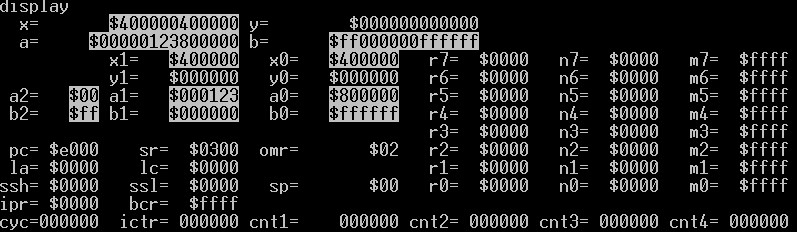
\includegraphics[scale=1]{figs/ej4/1.jpg}
    \caption{Carga inicial de los registros.}
    \label{fig:ej4_iniregs}
\end{figure}

\begin{figure}[H]
    \centering
    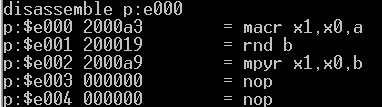
\includegraphics[scale=1]{figs/ej4/2.jpg}
    \caption{Carga de las instrucciones a ejecutar.}
    \label{fig:ej4_insts}
\end{figure}

\begin{figure}[H]
    \centering
    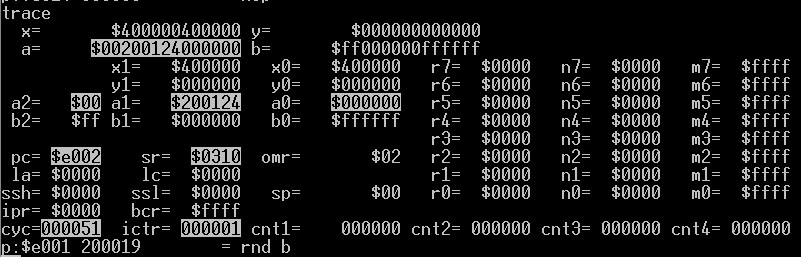
\includegraphics[scale=1]{figs/ej4/3.jpg}
    \caption{Primera instrucción ejecutada (macr x0,x1,a). }
    \label{fig:ej4_inst1}
\end{figure}

\begin{figure}[H]
    \centering
    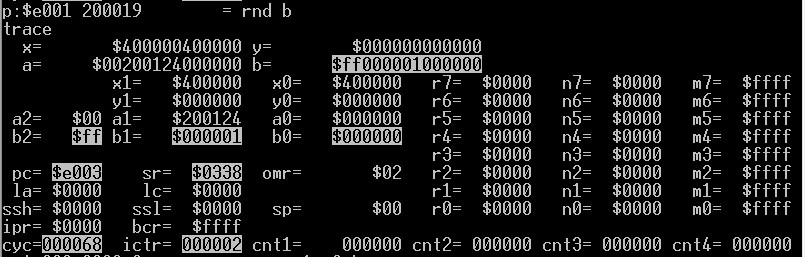
\includegraphics[scale=1]{figs/ej4/4.jpg}
    \caption{Segunda instrucción ejecutada (rnd b). }
    \label{fig:ej4_inst2}
\end{figure}

\begin{figure}[H]
    \centering
    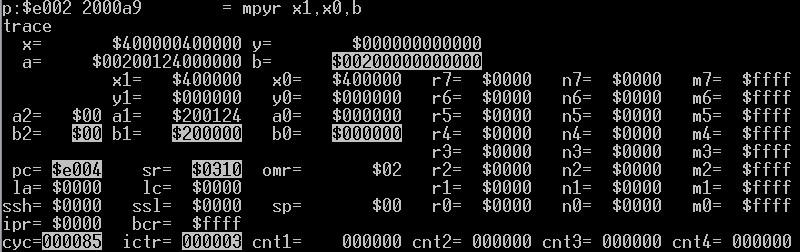
\includegraphics[scale=1]{figs/ej4/5.jpg}
    \caption{Última instrucción ejecutada (mpyr x0,x1,b). }
    \label{fig:ej4_inst3}
\end{figure}